\documentclass[12pt,twocolumn]{article}

\usepackage{algorithm}
\usepackage{algpseudocode}
\usepackage[margin=1in]{geometry}
\setlength{\parindent}{0pt}
\usepackage{graphicx}
\usepackage{anyfontsize}
\usepackage{amsmath}
\usepackage{booktabs}
\usepackage{titling}
\usepackage{float}
% Define custom title command to increase the title font size
\pretitle{\begin{center}\fontsize{24pt}{30pt}\selectfont\bfseries}
\posttitle{\par\end{center}\vskip 0.5em}

% Authors and affiliation formatting
\newcommand{\authorinfo}[3]{
    {\fontsize{12pt}{14pt}\selectfont \textit{#1}} \\ % Author name in italic
    {\fontsize{12pt}{14pt}\selectfont \textbf{#2}} \\ % Student ID in bold
    {\fontsize{12pt}{14pt}\selectfont \texttt{#3}} \vspace{1em} % Email in typewriter font
}

\begin{document}

% Title
\title{Comparison of merge sort and counting sort}
\date{} % Empty date

% Authors
\author{
    \authorinfo{Nafis Raihan Pial}{2003005}{2003005@student.ruetc.ac.bd} \and
    \authorinfo{Raihan Ul Islam}{200306}{2003006@student.ruetc.ac.bd} \and
    \authorinfo{Soscho Shamuel Gregory}{2003007}{2003007@student.ruetc.ac.bd} \and
    \authorinfo{Zabed Iqbal}{2003011}{2003011@student.ruetc.ac.bd} \and
    \authorinfo{MD. Sartaj Alam Pritom}{2003046}{2003046@student.ruetc.ac.bd} \and
    \authorinfo{Md. Shahidul Islam Dipu}{2003040}{2003040@student.ruetc.ac.bd}
}
\maketitle

% Rest of your document...
% Use the standard font size and style here, do not italicize unless specifically required.

\section{Abstract}
 The abstract entails a comparative analysis of Merge Sort and Counting Sort, emphasizing the assessment of their performance across a range of dataset sizes. The complexities, encompassing time complexities (Merge Sort: \(O(nlogn)\), Counting Sort: \(O(n+k))\), and space complexities are scrutinized. Notably, Merge Sort is highlighted for its adaptability to various datasets, while Counting Sort excels in linear efficiency, particularly well-suited for handling large datasets with restricted value ranges. The chosen methodology involves systematic experimentation with varying dataset sizes to provide empirical evidence on the sorting algorithms' performance. The findings contribute practical insights for real-world algorithm selection, with due consideration to acknowledged limitations related to dataset constraints. Recommendations include optimizing Merge Sort and exploring additional sorting algorithms. In conclusion, the abstract offers a succinct analysis that enriches sorting algorithm discussions for both researchers and practitioners.

\section{Introduction}
Sorting algorithms, the unsung heroes of computational efficiency, intricately shape the landscape of computer science applications. From database management to scientific computing and beyond, their impact on system performance is profound. In this research paper, we embark on a comprehensive exploration of two distinguished sorting algorithms—Merge Sort and Counting Sort. Our focus is to unravel the intricacies of these algorithms, shedding light on their respective strengths, weaknesses, and unique methodologies in organizing data.

\subsection{Significance of Sorting Algorithms}
The importance of efficient data organization and retrieval resonates across diverse domains of modern computing. Sorting algorithms serve as the linchpin of this organizational prowess, allowing for the seamless arrangement of elements and facilitating swift retrieval and analysis. As we traverse applications spanning web document searches to intricate financial transactions, sorting algorithms play a pivotal role in optimizing these computational processes.

Amidst the vast array of sorting algorithms, the need for diversity arises from the distinctive nature of datasets and the specific demands of various applications. No singular sorting technique can universally excel. Merge Sort, with its proven efficiency in dividing and conquering large datasets, contrasts with Counting Sort, a non-comparative algorithm adept at exploiting the inherent structure of data.

\subsection{Introducing Merge Sort and Counting Sort}
\textbf{Merge Sort:} Recognized for its elegance and reliability, Merge Sort is a divide-and-conquer algorithm celebrated for its efficient time complexity of \(O(n log n)\). In the realm of data organization, Merge Sort systematically breaks down datasets, skillfully sorts smaller segments, and seamlessly merges them to create ordered wholes. This meticulous process ensures not only intricately ordered data but also optimization for swift and efficient retrieval.
\\
\\
\textbf{Counting Sort:} An efficiency champion, Counting Sort distinguishes itself as a non-comparative algorithm, boasting a linear time complexity of \(O(n + k)\). Departing from conventional sorting methods, Counting Sort takes a statistical approach by counting the 
occurrences of distinct elements. This unique feature makes it exceptionally efficient, especially when dealing with datasets characterized by a limited range of values.

\subsection{Applications}
\textbf{Merge Sort:} Widely used in various applications, Merge Sort is particularly effective in scenarios where stable, efficient sorting is crucial. It is commonly employed in data processing, scientific computing, and any context demanding reliable sorting with a focus on maintaining order.
\\
\\
\textbf{Counting Sort:} Counting Sort shines in scenarios where datasets have a limited range of distinct values. Its efficiency becomes evident in applications such as sorting integers, character frequencies, or other scenarios where counting occurrences is beneficial. This sorting algorithm is frequently employed in data distribution analysis, enabling efficient calculations of frequencies.
\\
\\
In contrast to the illustrative imagery associated with Bubble Sort, these introductions aim to offer a succinct yet comprehensive overview of Merge Sort and Counting Sort. The added applications provide practical contexts, highlighting the strengths of each sorting algorithm in real-world scenarios.2.3 Objectives of this Study

\subsection{Objectives of this Study}
This research paper aims to conduct an exhaustive comparison between Merge Sort and Counting Sort. Through a meticulous exploration of their theoretical foundations and an empirical evaluation of their practical performance on diverse datasets, we seek to provide a nuanced understanding of the trade-offs and advantages inherent in each algorithm. By unraveling the dynamics of Merge Sort and Counting Sort, we strive to contribute valuable insights to the ongoing discussions surrounding algorithmic considerations in the realm of sorting algorithms.

\section{Background Study}
Sorting algorithms have been a subject of fascination in computer science, providing various solutions for efficient data organization. This study focuses on two significant contenders, Merge Sort and Counting Sort, aiming to unravel their algorithms, theoretical considerations, and applications.
\\
\\
\textbf{Merge Sort:}
Merge Sort, known for its elegance and stability, operates as a divide-and-conquer algorithm. Its efficiency shines through a time complexity of \(O(n log n)\), making it a reliable choice for sorting diverse datasets. Let's explore its algorithm breakdown and key theoretical aspects.
\cite{geeksforgeeks-merge-sort}
\\
\\

\begin{algorithm}[H]
\caption{Merge Sort Algorithm with Merge Procedure}\label{alg:merge_sort}
\begin{algorithmic}[1] % The number tells where the line numbering should start
\Procedure{Merge-Sort}{$A, p, r$}
    \If {$p < r$}
        \State $q = \left\lfloor (p + r) / 2 \right\rfloor$
        \State \Call{Merge-Sort}{$A, p, q$}
        \State \Call{Merge-Sort}{$A, q + 1, r$}
        \State \Call{Merge}{$A, p, q, r$}
    \EndIf
\EndProcedure
\Statex
\Procedure{Merge}{$A, p, q, r$}
    \State $n_1 = q - p + 1$
    \State $n_2 = r - q$
    \State Let $L[1..n_1 + 1]$ and $R[1..n_2 + 1]$ be new arrays
    \For {$i = 1$ to $n_1$}
        \State $L[i] = A[p + i - 1]$
    \EndFor
    \For {$j = 1$ to $n_2$}
        \State $R[j] = A[q + j]$
    \EndFor
    \State $L[n_1 + 1] = \infty$
    \State $R[n_2 + 1] = \infty$
    \State $i = 1$
    \State $j = 1$
    \For {$k = p$ to $r$}
        \If {$L[i] \leq R[j]$}
            \State $A[k] = L[i]$
            \State $i = i + 1$
        \Else
            \State $A[k] = R[j]$
            \State $j = j + 1$
        \EndIf
    \EndFor
\EndProcedure
\end{algorithmic}
\end{algorithm}
\cite{cormen2009introduction}
Merge Sort recursively dissects datasets, sorting smaller components, and seamlessly merges them back into wholes. This divide-and-conquer strategy ensures ordered data and optimization for efficient retrieval.
\clearpage

\begin{figure}
  \centering
  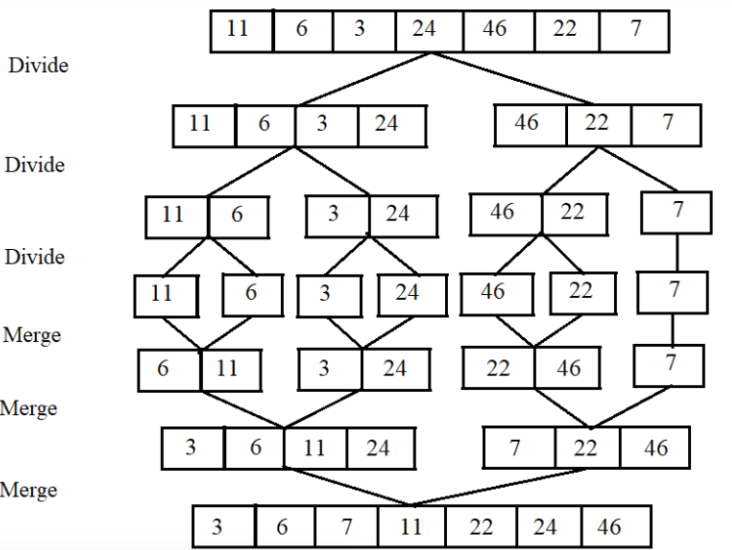
\includegraphics[width=0.8\linewidth]{image.png} 
  \caption{\textbf{Process}}
  \label{fig:my_label}
\end{figure}

\begin{enumerate}
  \item Time Complexity:
  \begin{itemize}
    \item Average-case: \( O(n \log n) \)
    \item Worst-case: \( O(n \log n) \)
  \end{itemize}
  
  \item Space Complexity: \( O(n) \)
  
  \item In-place Algorithm: No
  
  \item Stability: Merge Sort is not inherently stable. If two elements have the same key, their relative order might change after sorting.
\end{enumerate}

\textbf{Counting Sort:}
Counting Sort, a paradigm of efficiency, stands out as a non-comparative algorithm with a linear time complexity of O(n + k). This unique approach involves counting occurrences of distinct elements. Let's explore its algorithm breakdown and key theoretical aspects.
\cite{geeksforgeeks-counting-sort}
Arrays:
\begin{itemize}
    \item \( A[1, \ldots, n] \) original unsorted array
    \item \( B[1, \ldots, n] \) array to hold sorted output
    \item \( C[1, \ldots, k] \) working array to hold counts
\end{itemize}

\begin{algorithm}[H]
\caption{Counting Sort}\label{alg:counting_sort}
\begin{algorithmic}[1]
\Procedure{Counting\_Sort}{$A, B, k$}
    \State // initialize the count array
    \For{$i = 1$ to $k$}
        \State $C[i] = 0$
    \EndFor
    \For{$j = 1$ to \text{length}[A]}
        \State $C[A[j]] = C[A[j]] + 1$
    \EndFor
    \State // $C[i]$ now contains the number of elements equal to $i$.
    \For{$i = 2$ to $k$}
        \State $C[i] = C[i] + C[i - 1]$
    \EndFor
    \State // $C[i]$ now contains the number of elements less than or equal to $i$.
    \For{$j = \text{length}[A]$ downto $1$}
        \State $B[C[A[j]]] = A[j]$
        \State $C[A[j]] = C[A[j]] - 1$
    \EndFor
\EndProcedure
\end{algorithmic}
\end{algorithm}

Counting Sort begins by creating an array filled with zeros and counting occurrences of each distinct element. It then calculates positions for elements and efficiently places them in their final order
\cite{garg2017practical}
\\
\\
\textbf{Theoretical Considerations:}

\begin{enumerate}
  \item Time Complexity: \( O(n + k) \), where \( n \) is the number of elements, and \( k \) is the range of distinct values.
  \item Space Complexity: \( O(k) \), requires an auxiliary array of size \( k \).
  \item Stability: Stable – preserves the relative order of equal elements.
\end{enumerate}

\textbf{Comparative Analysis:}
The theoretical underpinnings provide insights into the strengths of each algorithm. Merge Sort offers versatility and stability, making it suitable for various datasets. Counting Sort, with its linear efficiency, excels in scenarios with a limited range of values.

In the comparative analysis, attention should be given to the distinct algorithm breakdowns, marked by the respective pictures. Merge Sort's divide-and-conquer strategy contrasts with Counting Sort's unique counting approach. Understanding the theoretical considerations guides the selection based on the dataset's characteristics.

This study aims to contribute to the ongoing discourse on sorting algorithms, providing a foundation for a thorough comparison between Merge Sort and Counting Sort. The upcoming sections will delve deeper into empirical evaluations and practical applications, offering a holistic view of their performance characteristics.

\section{Results and Analysis}
\subsection{Introduction to Results}
This experiment meticulously evaluates and compares the performance of Merge Sort and Counting Sort, two fundamental sorting algorithms. Sorting algorithms are integral in computer science and data processing, influencing the efficiency and speed of various applications. The primary goal of our study is to analyze how these algorithms perform across a spectrum of dataset sizes, ranging from small to significantly large datasets.
\subsubsection{Dataset Variation and Configuration}
To comprehensively understand the performance of the algorithms, datasets of varying sizes were configured, specifically including 10,000, 20,000, 30,000, 40,000, 50,000, 60,000, 70,000, 80,000, 90,000, and 100,000 data points. Each dataset was chosen to represent practical scenarios, ranging from everyday modest-sized datasets to more extensive datasets reflecting substantial data processing demands.
\paragraph{Results of the Sorting}
\textbf{Execution Times}
\\
\begin{tabular}{|c|c|c|}




\hline Data Size & \begin{tabular}{c} 




Merge Sort Time \\




(in miliseconds)




\end{tabular} & \begin{tabular}{c} 




Counting Sort Time \\




(in miliseconds)




\end{tabular} \\




\hline 10000 & 4074.8 & 534.5 \\




\hline 20000 & 8387.2 & 691.9 \\




\hline 30000 & 13791.6 & 979.9 \\




\hline 40000 & 17537.1 & 1141.7 \\




\hline 50000 & 22100.3 & 1336.2 \\




\hline 60000 & 26453.6 & 1571 \\




\hline 70000 & 31218.4 & 1709.2 \\




\hline 80000 & 35476 & 1955.8 \\




\hline 90000 & 40404.9 & 2691.7 \\




\hline 100000 & 45341.8 & 3288.1 \\




\hline




\end{tabular}


\cite{googlescholar}
The execution times for Merge Sort and Counting Sort on datasets of different sizes are presented below:
\subsubsection{The graph}
\begin{figure}[H]
  \centering
  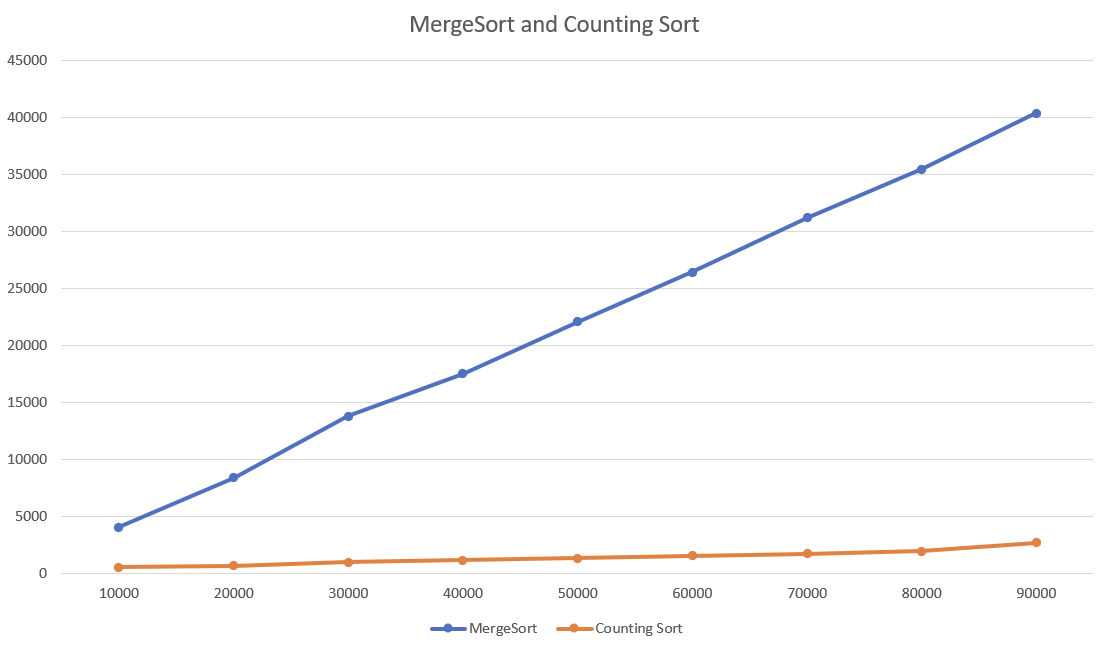
\includegraphics[width=1\linewidth]{mergeVcounting_1.png} 
  \caption{\textbf{Merge sort and counting sort}}
  \label{fig:my_label}
\end{figure}
\begin{figure}[H]
    \centering
    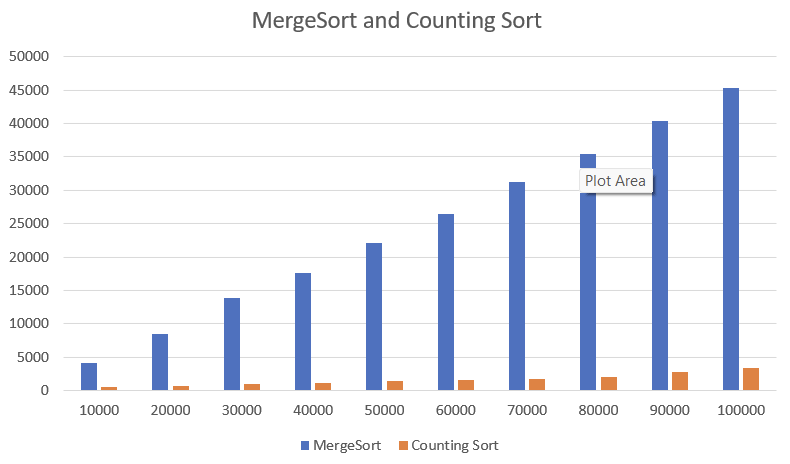
\includegraphics[width=1\linewidth]{mergeVcounting_2.png}
    \caption{\textbf{Merge sort and counting sort}}
    \label{fig:enter-label}
\end{figure}

\subsubsection{Analysis}
Comparing the time complexities of Merge Sort and Counting Sort provides valuable insights into their respective performance characteristics, especially concerning dataset size.
\cite{researchgate}
\cite{googlescholar}
\begin{enumerate}
    \item Observations:
    \begin{itemize}
        \item Merge Sort:
        \begin{itemize}
            \item Time increases consistently with the growth of the dataset.
            \item Reflects the expected behavior of \( O(n\log n) \) time complexity.
            \item Non-linear increase indicates the influence of the logarithmic factor.
        \end{itemize}
        \item Counting Sort:
        \begin{itemize}
            \item Demonstrates consistently lower times compared to Merge Sort.
            \item Reflects the expected behavior of \( O(n\log n) \) time complexity.
            \item Linear time complexity \(O(n+k)\) contributes to its efficiency, especially for smaller datasets.
        \end{itemize}
    \end{itemize}
    \item  Explanation:
        \begin{itemize}
        \item Merge Sort:
        \begin{itemize}
            \item Performs well but exhibits a logarithmic growth in time.
            \item Becomes relatively more efficient as dataset size increases.
        \end{itemize}
        \item Counting Sort:
        \begin{itemize}
            \item Maintains efficiency across all dataset sizes.
            \item Linear time complexity allows for faster sorting, especially for smaller datasets.
        \end{itemize}
    \end{itemize}
    \item  Recommendations:
        \begin{itemize}
        \item For Smaller Datasets:
        \begin{itemize}
            \item Counting Sort: Highly efficient due to its linear time complexity. Recommended for datasets with limited sizes.
        \end{itemize}
        \item For Larger Datasets:
        \begin{itemize}
            \item Merge Sort: Becomes a competitive and efficient choice as dataset size increases. Balances efficiency and stability for larger and more complex datasets.
        \end{itemize}
    \end{itemize}
    \item  Practical Implications:
        \begin{itemize}
        \item Merge Sort:
        \begin{itemize}
            \item Suitable for general-purpose sorting where stability and adaptability are crucial.
            \item Versatile, making it viable for diverse sorting requirements in manageable dataset sizes.
            \item Particularly beneficial when a stable sorting algorithm is required.
        \end{itemize}
        \item For Larger Datasets:
        \begin{itemize}
            \item Ideal for scenarios with a limited range of values.
            \item Efficient and scalable, particularly advantageous for large datasets.
            \item Well-suited for situations with a constrained range, prioritizing sorting speed over versatility.
        \end{itemize}
    \end{itemize}
\end{enumerate}

\section{Conclusions}
The comprehensive comparison between Merge Sort and Counting Sort has illuminated their distinct characteristics. Merge Sort, though stable, demonstrated limitations in efficiency for larger or complex datasets, aligning with its expected time complexity growth \(O(nlogn)\). Counting Sort's linear time complexity \((O(n+k))\) showcased remarkable efficiency, particularly excelling in scenarios with large datasets. The findings endorse Counting Sort as a preferred choice for fast sorting in applications prioritizing sorting speed. Its adaptability to diverse real-world scenarios offers valuable insights for algorithm selection. The study underscores the significance of considering algorithmic characteristics and real-world requirements when choosing sorting methods, ultimately guiding towards informed and effective decision-making.

\bibliographystyle{plain}
\bibliography{refs}


\end{document}

